\documentclass[11pt]{beamer}
\usepackage[utf8]{inputenc}
\usepackage[T1]{fontenc}
\usepackage{tikz}
\usepackage{amsmath}
\usepackage{amsfonts}
\usepackage{amssymb}
\usepackage{graphicx}
\usetheme{default}
\usepackage{tikz}
\usetikzlibrary{shapes,arrows}
% Define block styles
\tikzstyle{decision} = [diamond, draw, fill=blue!20, 
text width=4.5em, text badly centered, node distance=3cm, inner sep=0pt]
\tikzstyle{block} = [rectangle, draw, fill=blue!20, text width=5em, text centered, rounded corners, minimum height=4em]
\tikzstyle{line} = [draw, -latex']
\tikzstyle{cloud} = [draw, ellipse,fill=red!20, node distance=3cm,
minimum height=2em]
\begin{document}
	\author{Bradley Gram-Hansen}
	\title{An overview of results}
	%\subtitle{}
	%\logo{}
	%\institute{}
	%\date{}
	%\subject{}
	%\setbeamercovered{transparent}
	%\setbeamertemplate{navigation symbols}{}
	\frame[plain]{\maketitle}
	
	\begin{frame}
		\frametitle{Models}
		\begin{itemize}
			\item Recursive, single input Gaussian process model
		\end{itemize}
   \begin{figure}
   \scalebox{0.5}{
	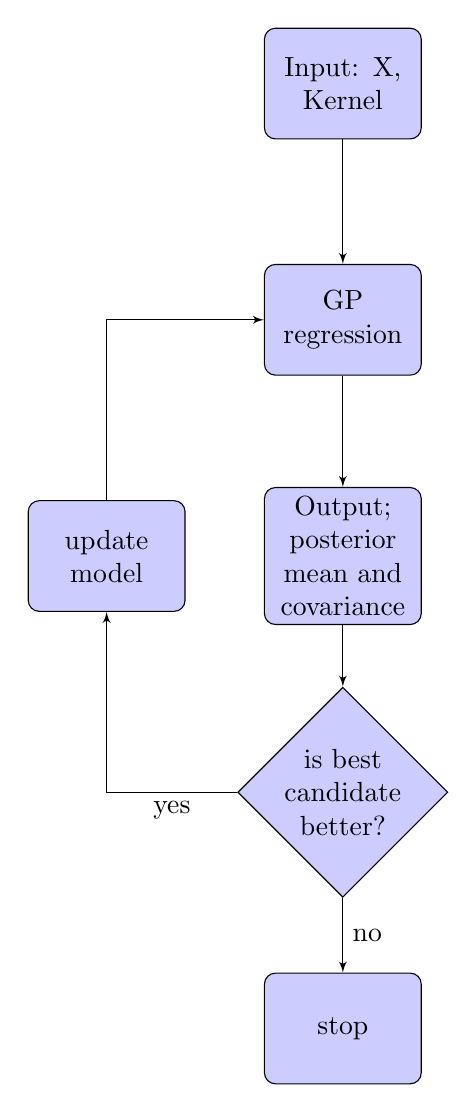
\begin{tikzpicture}[node distance = 3cm, auto]
	% Place nodes
	\node [block] (init) {Input: X, Kernel};
%	\node [cloud, left of=init] (expert) {input: kernel, X};
%	\node [cloud, right of=init] (system) {input X};
	\node [block, below of=init] (regression) {GP regression};
	\node [block, below of=regression] (evaluate) {Output; posterior mean and covariance};
	\node [block, left of=evaluate, node distance=3cm] (update) {update model};
	\node [decision, below of=evaluate] (decide) {is best candidate better?};
	\node [block, below of=decide, node distance=3cm] (stop) {stop};
	% Draw edges
	\path [line] (init) -- (regression);
	\path [line] (regression) -- (evaluate);
	\path [line] (evaluate) -- (decide);
	\path [line] (decide) -| node [near start] {yes} (update);
	\path [line] (update) |- (regression);
	\path [line] (decide) -- node {no}(stop);
%	\path [line,dashed] (expert) -- (init);
%	\path [line,dashed] (system) -- (init);
%	\path [line,dashed] (system) |- (evaluate);
	\end{tikzpicture}
}\end{figure}
	\end{frame}
\end{document}